\documentclass{standalone}
\usepackage{tikz}
\usetikzlibrary{arrows.meta}

\begin{document}

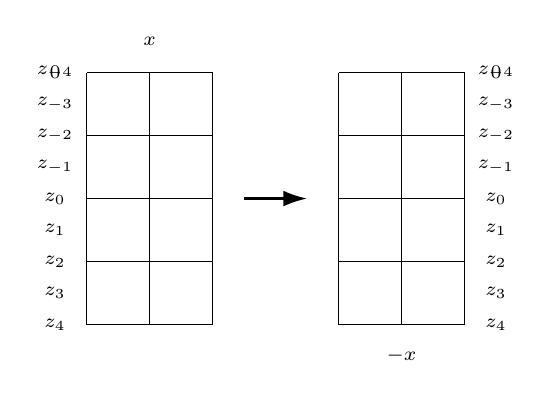
\begin{tikzpicture}[scale=0.8, every node/.style={font=\scriptsize}]

  % Left grid
  \draw (-3,2) grid (-1,-2);
  \foreach \i [count=\j from -4] in {0,...,8}
    \node at (-3.5,2-\i/2) {$z_{\j}$};
  \node at (-2,2.5) {$x$};
  \node at (-3.5,2) {$0$};
  
  % Right grid
  \draw (1,2) grid (3,-2);
  \foreach \i [count=\j from -4] in {0,...,8}
    \node at (3.5,2-\i/2) {$z_{\j}$};
  \node at (2,-2.5) {$-x$};
  \node at (3.5,2) {$0$};
  
  % Arrow between grids
  \draw[-{Latex[length=3mm,width=2mm]}, line width=0.8pt] (-0.5,0) -- (0.5,0);

\end{tikzpicture}

\end{document}